\chapter{Project Planning and Management}
\label{chap:project_planning}

This chapter outlines the strategic framework governing the development of the \textbf{Questro} recommendation system. It details the project's objectives, the adopted Systems Development Life Cycle (SDLC) methodology, and the rigorous scheduling of distinct phases from July 2025 through June 2026. Furthermore, it analyzes potential risks and establishes a comprehensive plan for resource allocation and quality assurance throughout the project lifecycle.

\section{Project Objectives}
\label{sec:project_objectives}
The planning phase begins by defining clear, measurable goals for the system. The primary objective is the \textbf{functional delivery} of a cross-domain web application that integrates a hybrid recommendation engine with user reviews and social features. To achieve this, the project focuses on \textbf{task decomposition}, dividing the complex system into manageable, modular components such as the AI model, .NET Backend API, and React Frontend. Strict \textbf{milestone planning} is employed to ensure the timely delivery of each phase.

\section{Project Phases}
\label{sec:project_phases}
The project lifecycle follows a structured SDLC approach. To ensure flexibility and continuous improvement, the project progresses through the following distinct phases, as visualized in the project's master schedule.

\subsection{Project Initiation and Planning}
\label{subsec:initiation}
The project commenced with a strictly defined initiation phase (July 1, 2025 – August 25, 2025). This phase focused on defining the problem scope, selecting the technical stack (\textbf{.NET, React, and Python}), and preparing the formal project proposal. As shown in Figure \ref{fig:planning_schedule}, this phase concluded with the approval of the proposal.

\begin{figure}[H]
    \centering
    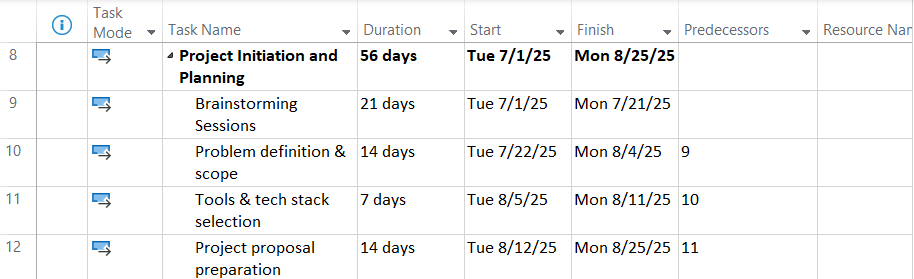
\includegraphics[width=1\textwidth]{figures/projectTimeLine/project-planning.png}
    \caption{Project Initiation and Planning Schedule (July 2025 – August 2025)}
    \label{fig:planning_schedule}
\end{figure}

\subsection{System Analysis}
\label{subsec:system_analysis}
Following initiation, the System Analysis phase (August 26, 2025 – October 13, 2025) established the foundation for the project. This 49-day phase involved gathering functional requirements regarding movies, games, and user profiles. Concurrently, a robust \textbf{data strategy} was defined to clean and structure datasets. Architectural modeling was performed to prepare Use Case and Activity diagrams, as detailed in Figure \ref{fig:analysis_schedule}.

\begin{figure}[H]
    \centering
    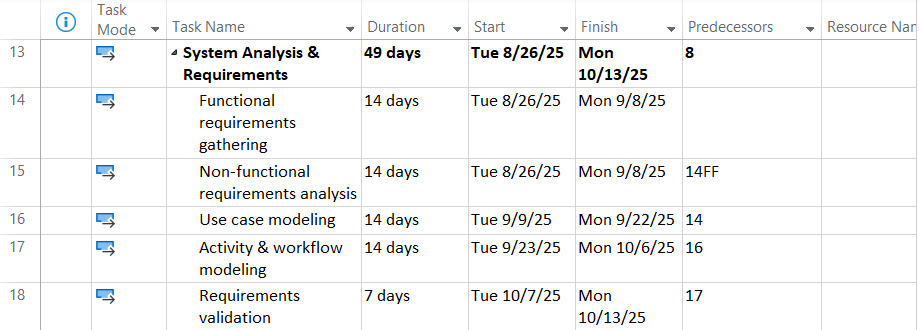
\includegraphics[width=1\textwidth]{figures/projectTimeLine/system-analythis.png}
    \caption{System Analysis and Requirements Timeline}
    \label{fig:analysis_schedule}
\end{figure}

\subsection{System Design and Architecture}
\label{subsec:design}
The Design phase (October 14, 2025 – December 1, 2025) bridged the gap between requirements and implementation. This phase included:
\begin{itemize}
    \item \textbf{UI/UX Wireframing:} Designing the visual interface and user journeys.
    \item \textbf{Database Design:} Defining the ERD and schemas for the Movie and Game datasets.
    \item \textbf{Backend Architecture:} Establishing .NET API endpoints and authentication flows.
\end{itemize}

\begin{figure}[H]
    \centering
    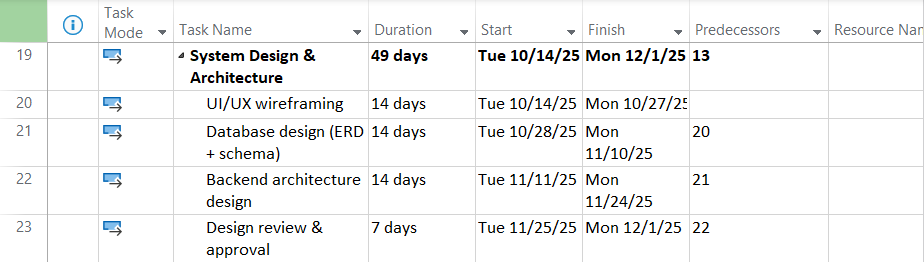
\includegraphics[width=1\textwidth]{figures/projectTimeLine/system-design.png}
    \caption{System Design and Architecture Timeline}
    \label{fig:design_schedule}
\end{figure}

\subsection{Development}
\label{subsec:development}
The development phase is the core of the project implementation. To maximize efficiency, the engineering effort was divided into two parallel tracks starting in mid-January 2026: \textbf{Backend/AI} and \textbf{Frontend}.

\subsubsection{Backend and AI Development}
Running from January 16, 2026, to March 24, 2026, this track focused on constructing the recommendation engine utilizing hybrid techniques. Tasks included dataset collection, feature engineering, and the implementation of the "Cold Start" strategy. Parallel to the AI work, the logic layer was built using \textbf{.NET} to ensure robust performance and type safety for the REST APIs.

\begin{figure}[H]
    \centering
    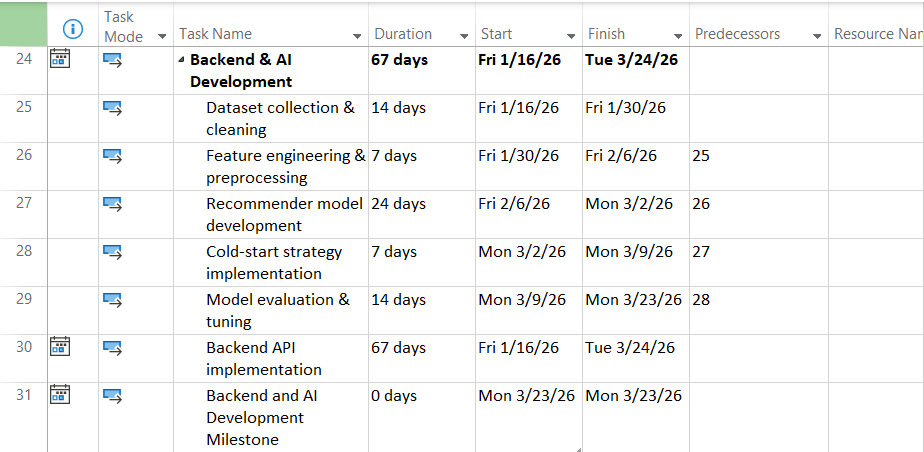
\includegraphics[width=1\textwidth]{figures/projectTimeLine/backend-and-ai.png}
    \caption{Backend and AI Development Schedule}
    \label{fig:backend_schedule}
\end{figure}

\subsubsection{Frontend Development}
Synchronized with the backend, the Frontend phase (January 16, 2026 – March 24, 2026) involved building the client-side application using \textbf{React} and \textbf{Bootstrap}. Key milestones included the development of UI components, authentication forms, and the integration of social features.

\begin{figure}[H]
    \centering
    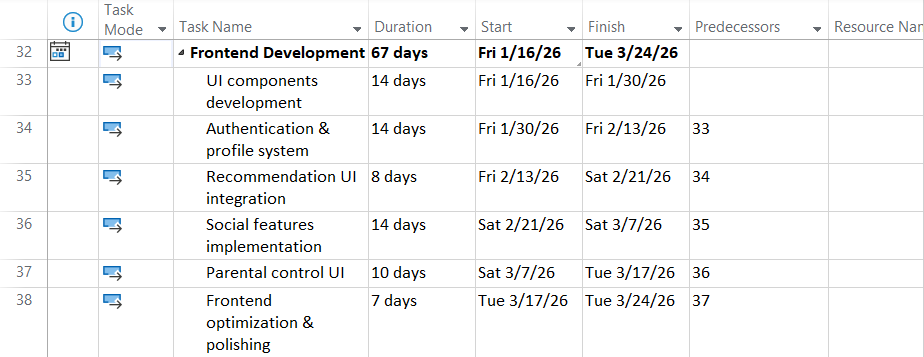
\includegraphics[width=1\textwidth]{figures/projectTimeLine/frontend.png}
    \caption{Frontend Development Schedule}
    \label{fig:frontend_schedule}
\end{figure}

\subsection{System Integration}
\label{subsec:integration}
Following the separate development tracks, the System Integration phase (March 24, 2026 – April 28, 2026) focused on linking the React Frontend with the .NET Backend APIs and the ML model. This phase ensured seamless data flow between the user interface and the recommendation logic, culminating in the Achievement Milestone.

\begin{figure}[H]
    \centering
    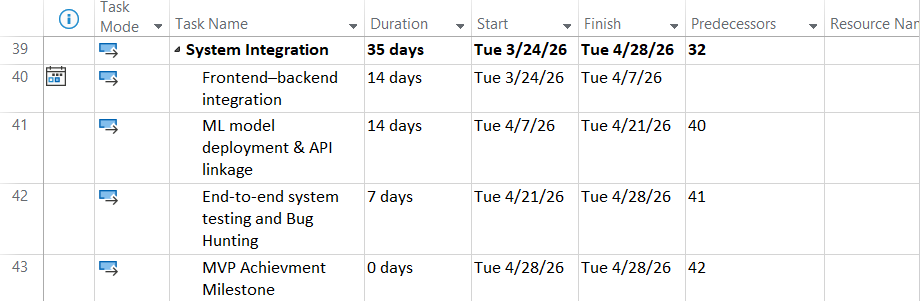
\includegraphics[width=1\textwidth]{figures/projectTimeLine/system-integration.png}
    \caption{System Integration Timeline}
    \label{fig:integration_schedule}
\end{figure}

\subsection{Testing and Quality Assurance}
\label{subsec:testing}
The final engineering phase (April 28, 2026 – June 2, 2026) ensures the system meets quality standards. This includes unit testing for individual components, integration testing, and performance optimization. User testing is scheduled for May 2026 to validate flows such as searching and generating recommendations.

\begin{figure}[H]
    \centering
    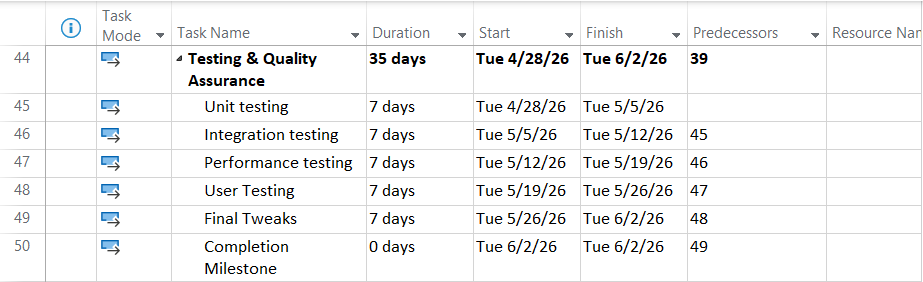
\includegraphics[width=1\textwidth]{figures/projectTimeLine/testing.png}
    \caption{Testing and Quality Assurance Schedule}
    \label{fig:testing_schedule}
\end{figure}

\subsection{Documentation}
\label{subsec:documentation}
While documentation is an ongoing process throughout the SDLC, the final compilation and drafting of the technical report and user manuals are scheduled for May and June 2026, ensuring the system is maintainable and usable upon delivery.

\begin{figure}[H]
    \centering
    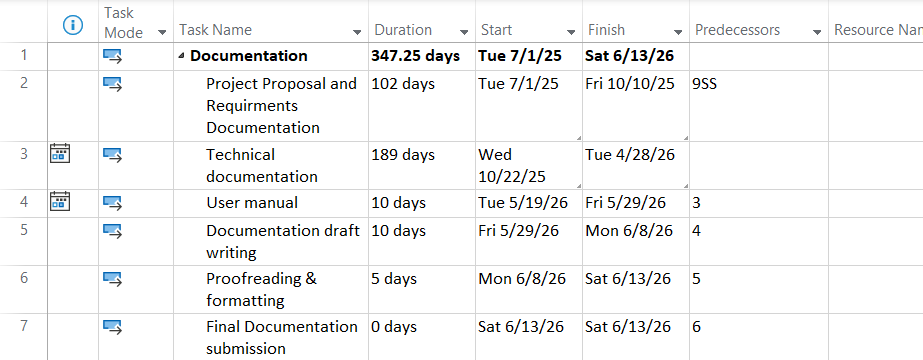
\includegraphics[width=1\textwidth]{figures/projectTimeLine/documentation-writing.png}
    \caption{Documentation Schedule}
    \label{fig:docs_schedule}
\end{figure}

\section{Risk Analysis}
\label{sec:risk_analysis}
Risk management is critical for minimizing the impact of uncertainties. The risks identified for this system are categorized as follows:

\subsection{Scheduling Risks}
\label{subsec:scheduling_risks}
Scheduling risks primarily involve potential delays in the project timeline. A significant factor is \textbf{algorithm tuning}, as the hybrid recommendation engine may require more iteration time than anticipated to reach acceptable accuracy. Additionally, \textbf{dependency issues} regarding third-party APIs (e.g., TMDB \cite{tmdb_ref} or IGDB \cite{igdb_ref}) could extend the development duration.

\subsection{Requirements Risks}
\label{subsec:requirements_risks}
Risks related to scope definition include \textbf{scope creep}, where the temptation to add non-core features like chat systems could dilute the project's focus. There is also potential \textbf{ambiguity} in defining the mathematical function for cross-domain recommendations.

\subsection{Technical Risks}
\label{subsec:technical_risks}
Technical risks pertain to the engineering challenges of the system. The primary concern is \textbf{data sparsity} (the "Cold Start" problem). Furthermore, \textbf{scalability} remains a risk if the dataset grows significantly during testing, potentially causing performance bottlenecks.

\section{Chapter Summary}
\label{sec:planning_summary}
In this chapter, we defined the project's core objectives and outlined a phased development approach based on the SDLC model. We detailed the strategies for system analysis, design, and implementation, supported by specific timelines and Gantt charts. Furthermore, we identified critical scheduling and technical risks. This planning phase establishes the operational framework for the project, paving the way for the \textbf{Related Work} investigation and subsequent \textbf{System Analysis} phases.